\documentclass[10pt]{article}
\usepackage[utf8]{inputenc}
\usepackage[T1]{fontenc}
\usepackage{amsmath}
\usepackage{amsfonts}
\usepackage{amssymb}
\usepackage[version=4]{mhchem}
\usepackage{stmaryrd}
\usepackage{graphicx}
\usepackage[export]{adjustbox}
\graphicspath{ {./images/} }

\begin{document}
\section*{CT1 Exercises for Control Structures}
\section*{Content}
CT1 Exercises for Control Structures ..... 1\\
Exercise 1 - Selection/Branch ..... 2\\
Exercise 2 - For-Loops ..... 3\\
Exercise 3 - From Code to Structogram ..... 4\\
Solutions ..... 5

\section*{Exercise 1 - Selection/Branch}
Encode the following Structograms into Flowchart, C- and ARM Assembly-language\\
A) If-Then-Else with unsigned 8-bit variables

\begin{center}
\begin{tabular}{|c|c|}
\hline
$n r X=n r Y$ & else \\
\hline
then $(n r X>n r Y)$ &  \\
\hline
\end{tabular}
\end{center}

B) If-Then-Else with signed 8-bit variables

\begin{center}
\begin{tabular}{|c|c|c|}
\hline
\multicolumn{3}{|l|}{\(
\text { then } \quad \text { if }(\operatorname{varA}<-17 \text { AND }
\)} \\
\hline
$\operatorname{varA}=-\operatorname{varB}$ &  & varB \\
\hline
\end{tabular}
\end{center}

C) If-Then-Else with signed 16-bit variables

\begin{center}
\begin{tabular}{|c|c|}
\hline
 & \multicolumn{3}{|c|}{\begin{tabular}{l}
if $(\operatorname{varC}=2344$ OR \\
$\operatorname{varC}>6788)$ \\
\end{tabular}} \\
\hline
then & else &  &  \\
\hline
$\operatorname{varC}=\operatorname{varC} / 4$ & $\operatorname{varC}=\operatorname{varC} / 2$ &  &  \\
\hline
\end{tabular}
\end{center}

\section*{Exercise 2 - For-Loops}
A) Write a for-loop in C- and ARM Assembly-language.\\
B) Compare your Assembly-language implementation with the compiler generated one. Hint: In the Keil uVision5 IDE

\begin{enumerate}
  \item create an empty C-language project (according to the respective introduction documents)
  \item add the C-language for-loop to the empty main function
  \item compile the project
  \item set a breakpoint in at the first line of the main function
  \item start debugging the program and let it run into the breakpoint
  \item compare your Assembly-language implementation of the for-loop with the compiler generated one
\end{enumerate}

Hint: for the purpose of this exercise, define your variables global and as "volatile" this tells the compiler to not optimize away the access to the variables since they are not used otherwise.

\section*{Exercise 3 - From Code to Structogram}
A) Analyze the following Assembly-language code and derive from this the matching structogram.\\
B) What result is stored in "outstr"?

\begin{verbatim}
    AREA progCode, CODE, READONLY
    THUMB
main
    PROC
    EXPORT main
    LDR R0,=srcstr
    LDR R1,=outstr
    MOVS R2,#0
cond LDRB R3,[R0,R2]
    CMP R3,#0
    BEQ endloop
    CMP R3,#60
    BLO store
    CMP R3,#90
    BHI store
    ADDS R3,R3,#32
store STRB R3,[R1,R2]
    ADDS R2,R2,#1
    B cond
endloop STRB R3,[R1,R2]
endless B endless
srcstr DCB "This IS mY TestStriNG", 0
    AREA progData, DATA, READWRITE
outstr SPACE 50
    END
\end{verbatim}

\section*{Solutions}
\section*{Exercise 1:}
A) If-Then-Else with unsigned 8-bit variables\\
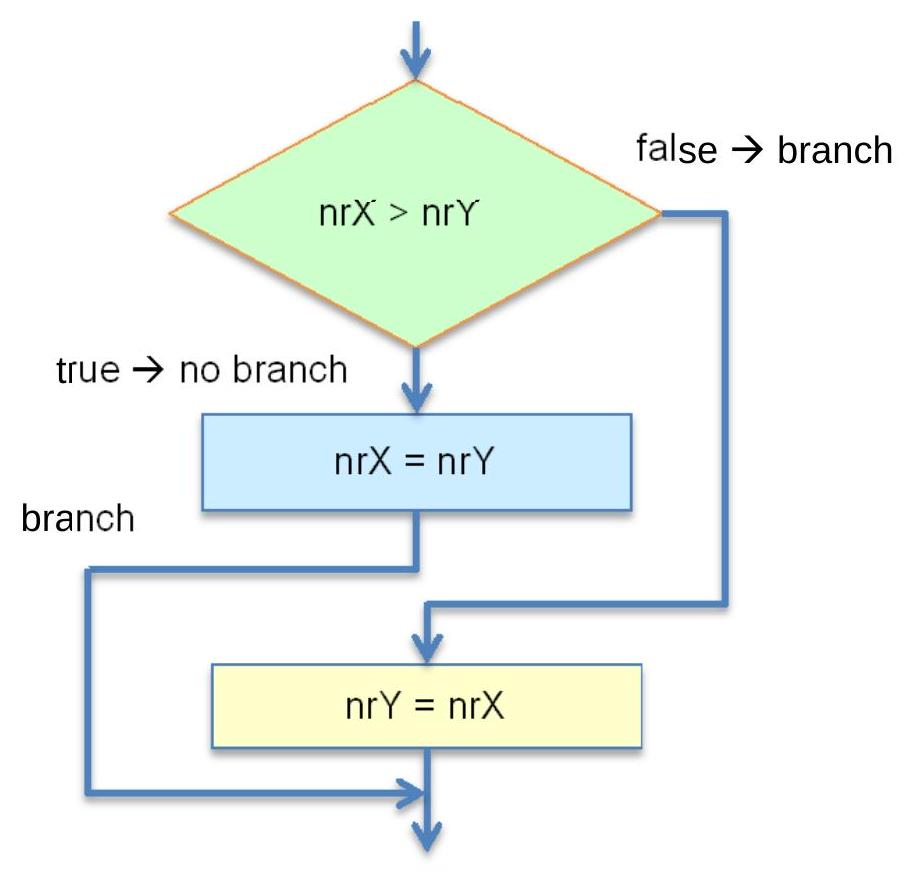
\includegraphics[width=\linewidth]{images/2025_01_02_7eee2d56b23c0199f878g-5}\\
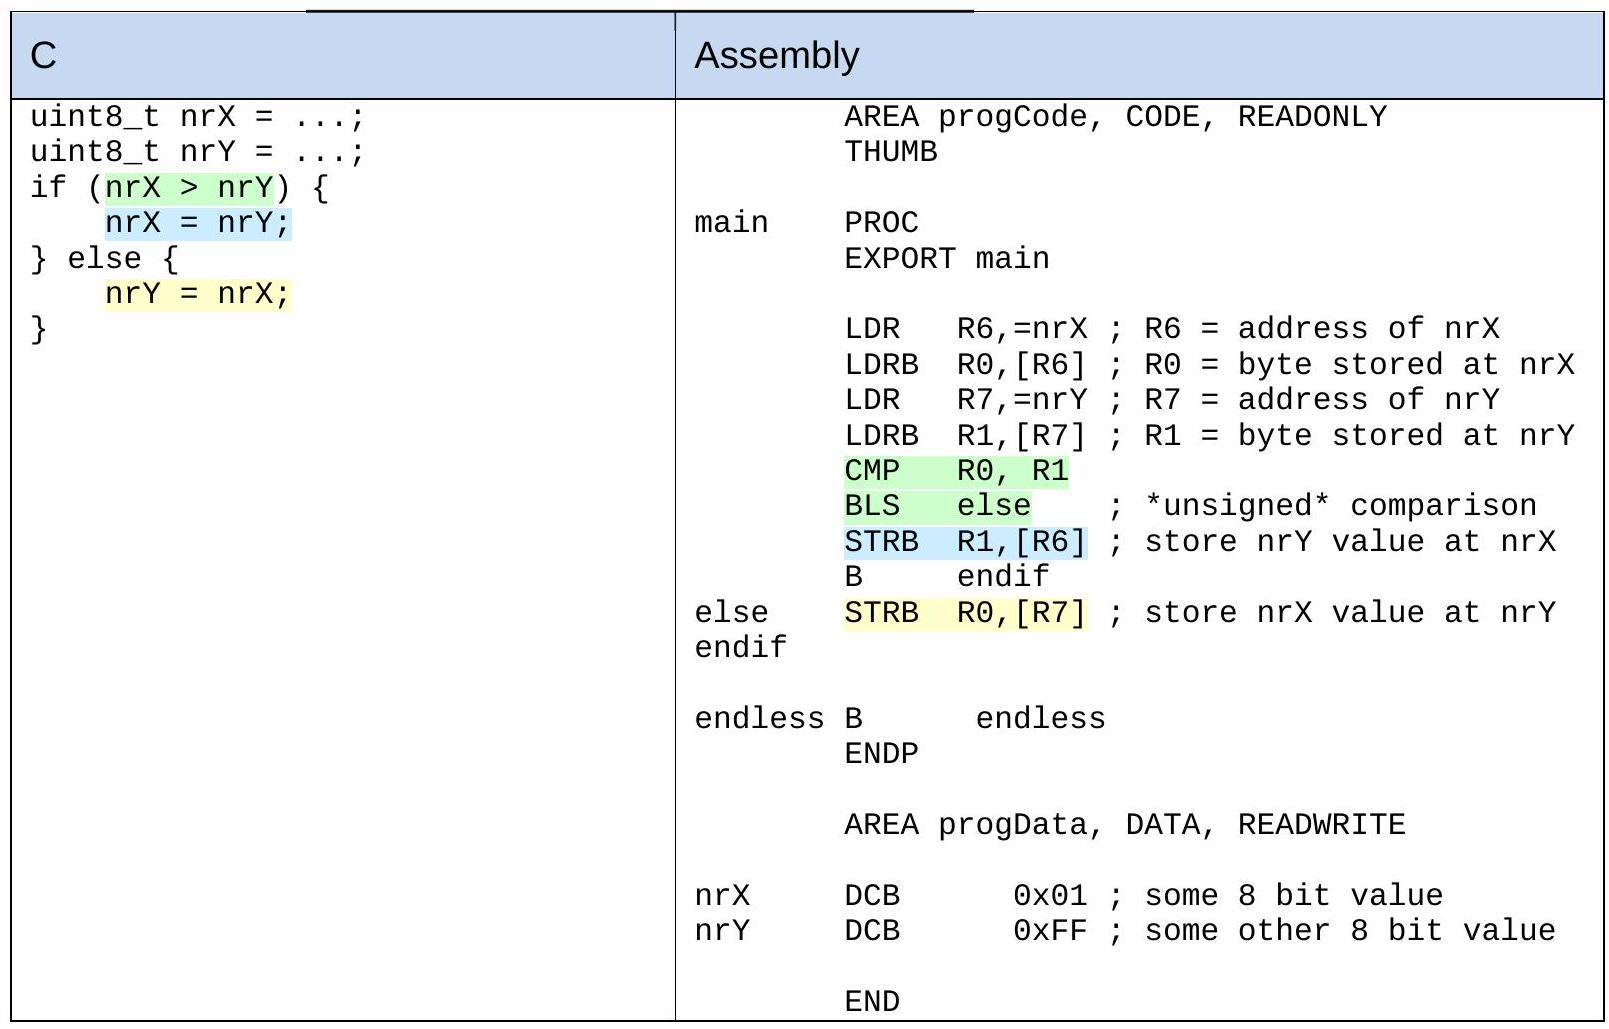
\includegraphics[width=\linewidth]{images/2025_01_02_7eee2d56b23c0199f878g-5(1)}\\
B) If-Then-Else with signed 8-bit variables\\
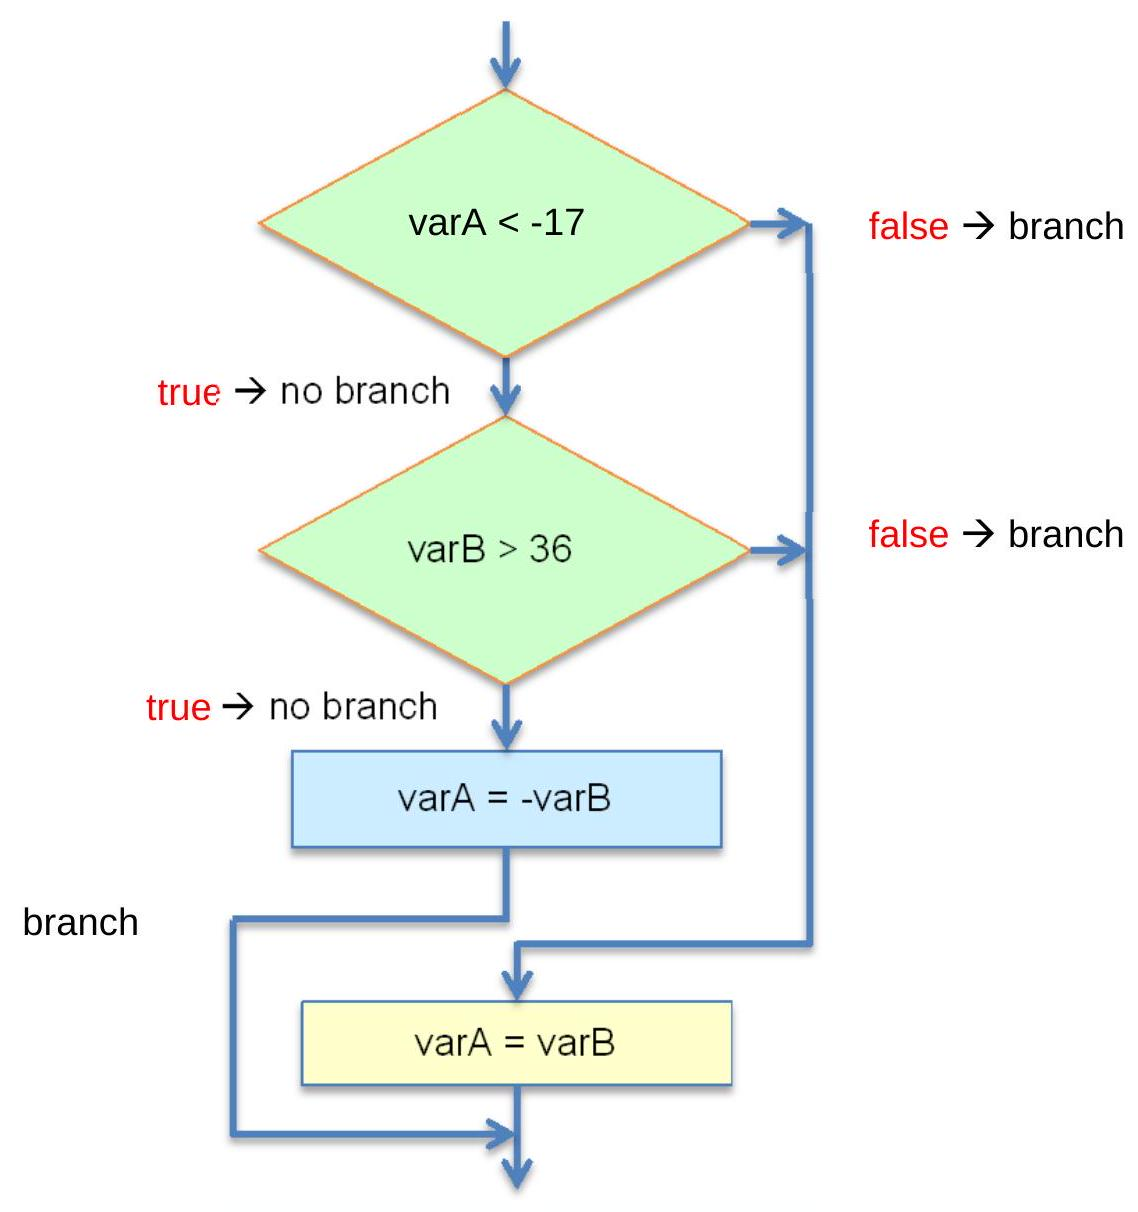
\includegraphics[width=\linewidth]{images/2025_01_02_7eee2d56b23c0199f878g-6}\\
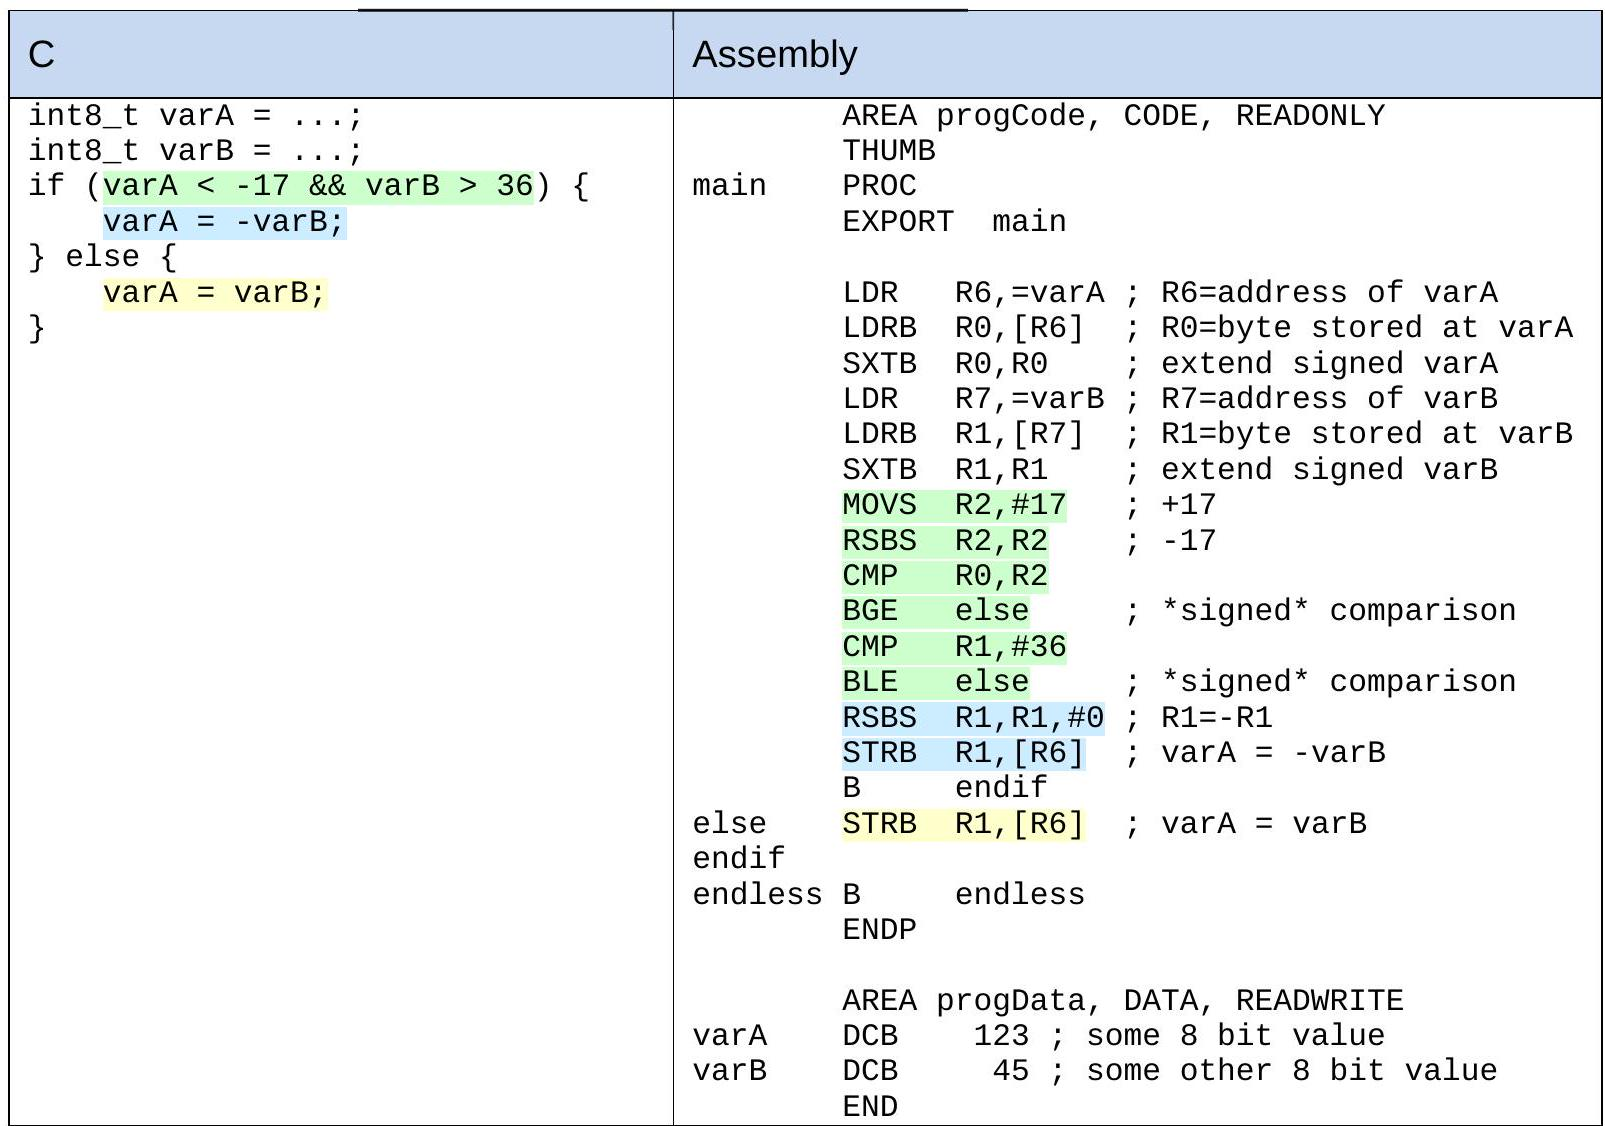
\includegraphics[width=\linewidth]{images/2025_01_02_7eee2d56b23c0199f878g-6(1)}\\
C) If-Then-Else with signed 16-bit variables\\
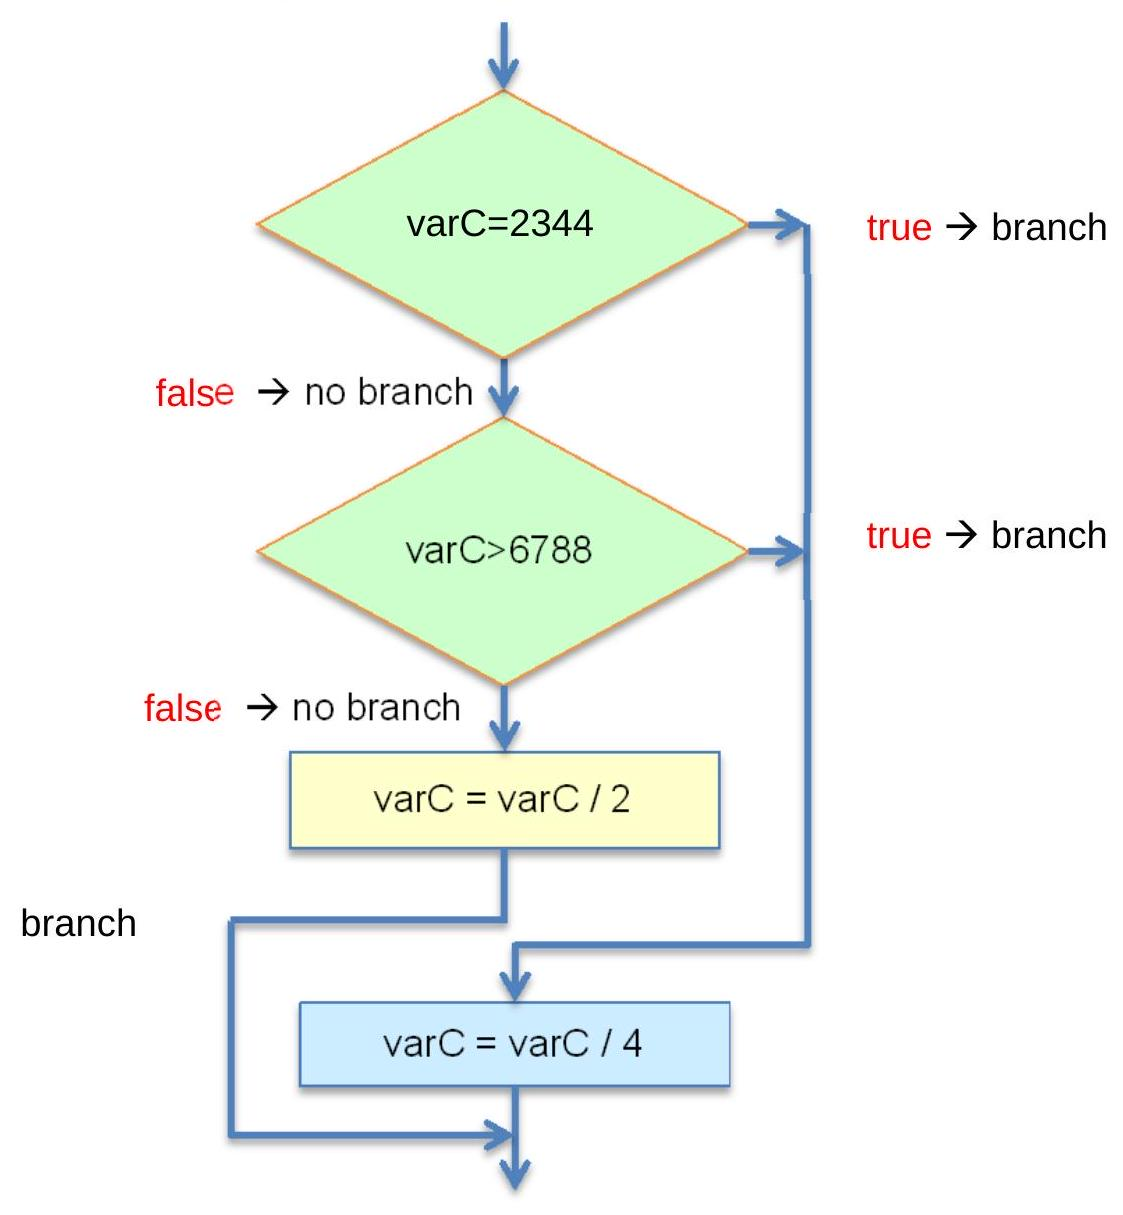
\includegraphics[width=\linewidth]{images/2025_01_02_7eee2d56b23c0199f878g-7(1)}

\begin{center}
\begin{tabular}{|c|c|}
\hline
C & Assembly \\
\hline
\texttt{int16\_t varC = ...; if (varC == 2344 || varC > 6788)\{ varC = varC / 4; \} else \{ varC = varC / 2; \}} & 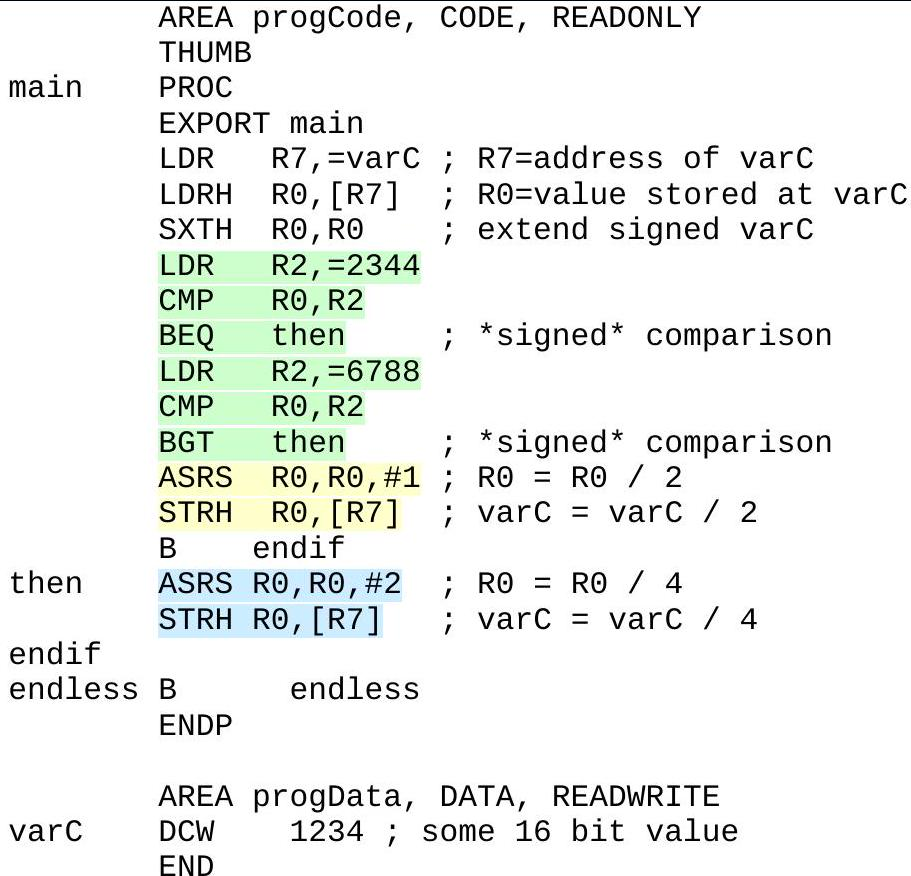
\includegraphics[width=\linewidth]{images/2025_01_02_7eee2d56b23c0199f878g-7}
 \\
\hline
\end{tabular}
\end{center}

\section*{Exercise 2:}
A) For-loop

\begin{center}
\begin{tabular}{|c|c|}
\hline
C & Assembly \\
\hline
\texttt{\#include <utils\_ctboard.h> \#include <stdint.h> ... int32\_t = 0; int32\_t count = 0; for(i = 0; i < 10; i++) \{ count++; \}} & 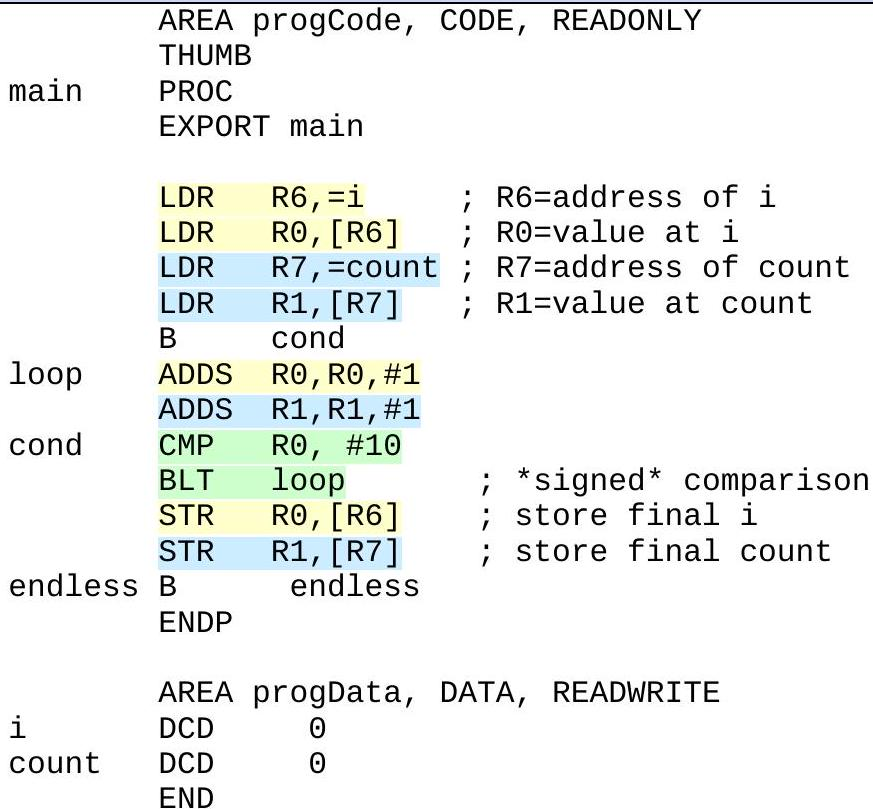
\includegraphics[width=\linewidth]{images/2025_01_02_7eee2d56b23c0199f878g-8}
 \\
\hline
\end{tabular}
\end{center}

B) Compare hand-crafted Assembly version to generated Assembly version\\
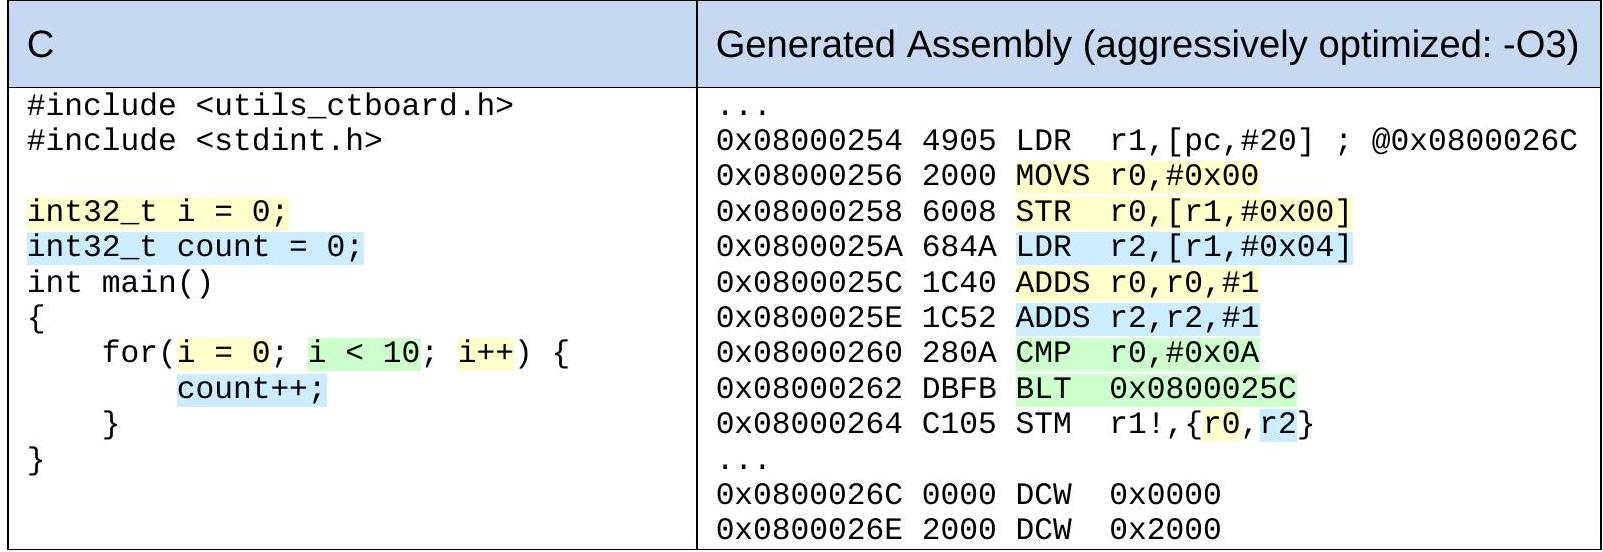
\includegraphics[width=\linewidth]{images/2025_01_02_7eee2d56b23c0199f878g-8(1)}

\section*{Exercise 3:}
A) The structorgram is

\begin{center}
\begin{tabular}{|c|c|}
\hline
\multicolumn{2}{|r|}{$\mathrm{R} 2=0$} \\
\hline
\multicolumn{2}{|l|}{while (R3 = srcstr[R2]) ! $=0$} \\
\hline
\multicolumn{2}{|l|}{\begin{tabular}{l}
\( \text { if (R3 >= } 60 \text { AND R3 <= 90) } \) \\
then else \\
\end{tabular}} \\
\hline
$\mathrm{R} 3=\mathrm{R} 3+32$ &  \\
\hline
\multicolumn{2}{|r|}{outstr[R2] = R3} \\
\hline
\multicolumn{2}{|r|}{INC R2} \\
\hline
\multicolumn{2}{|r|}{outstr[R2] = R3} \\
\hline
\end{tabular}
\end{center}

B) The resulting text is a null terminated string of all caps from the original string: THIS IS MY TESTSTRING


\end{document}